\begin{figure}
    \begin{center}
    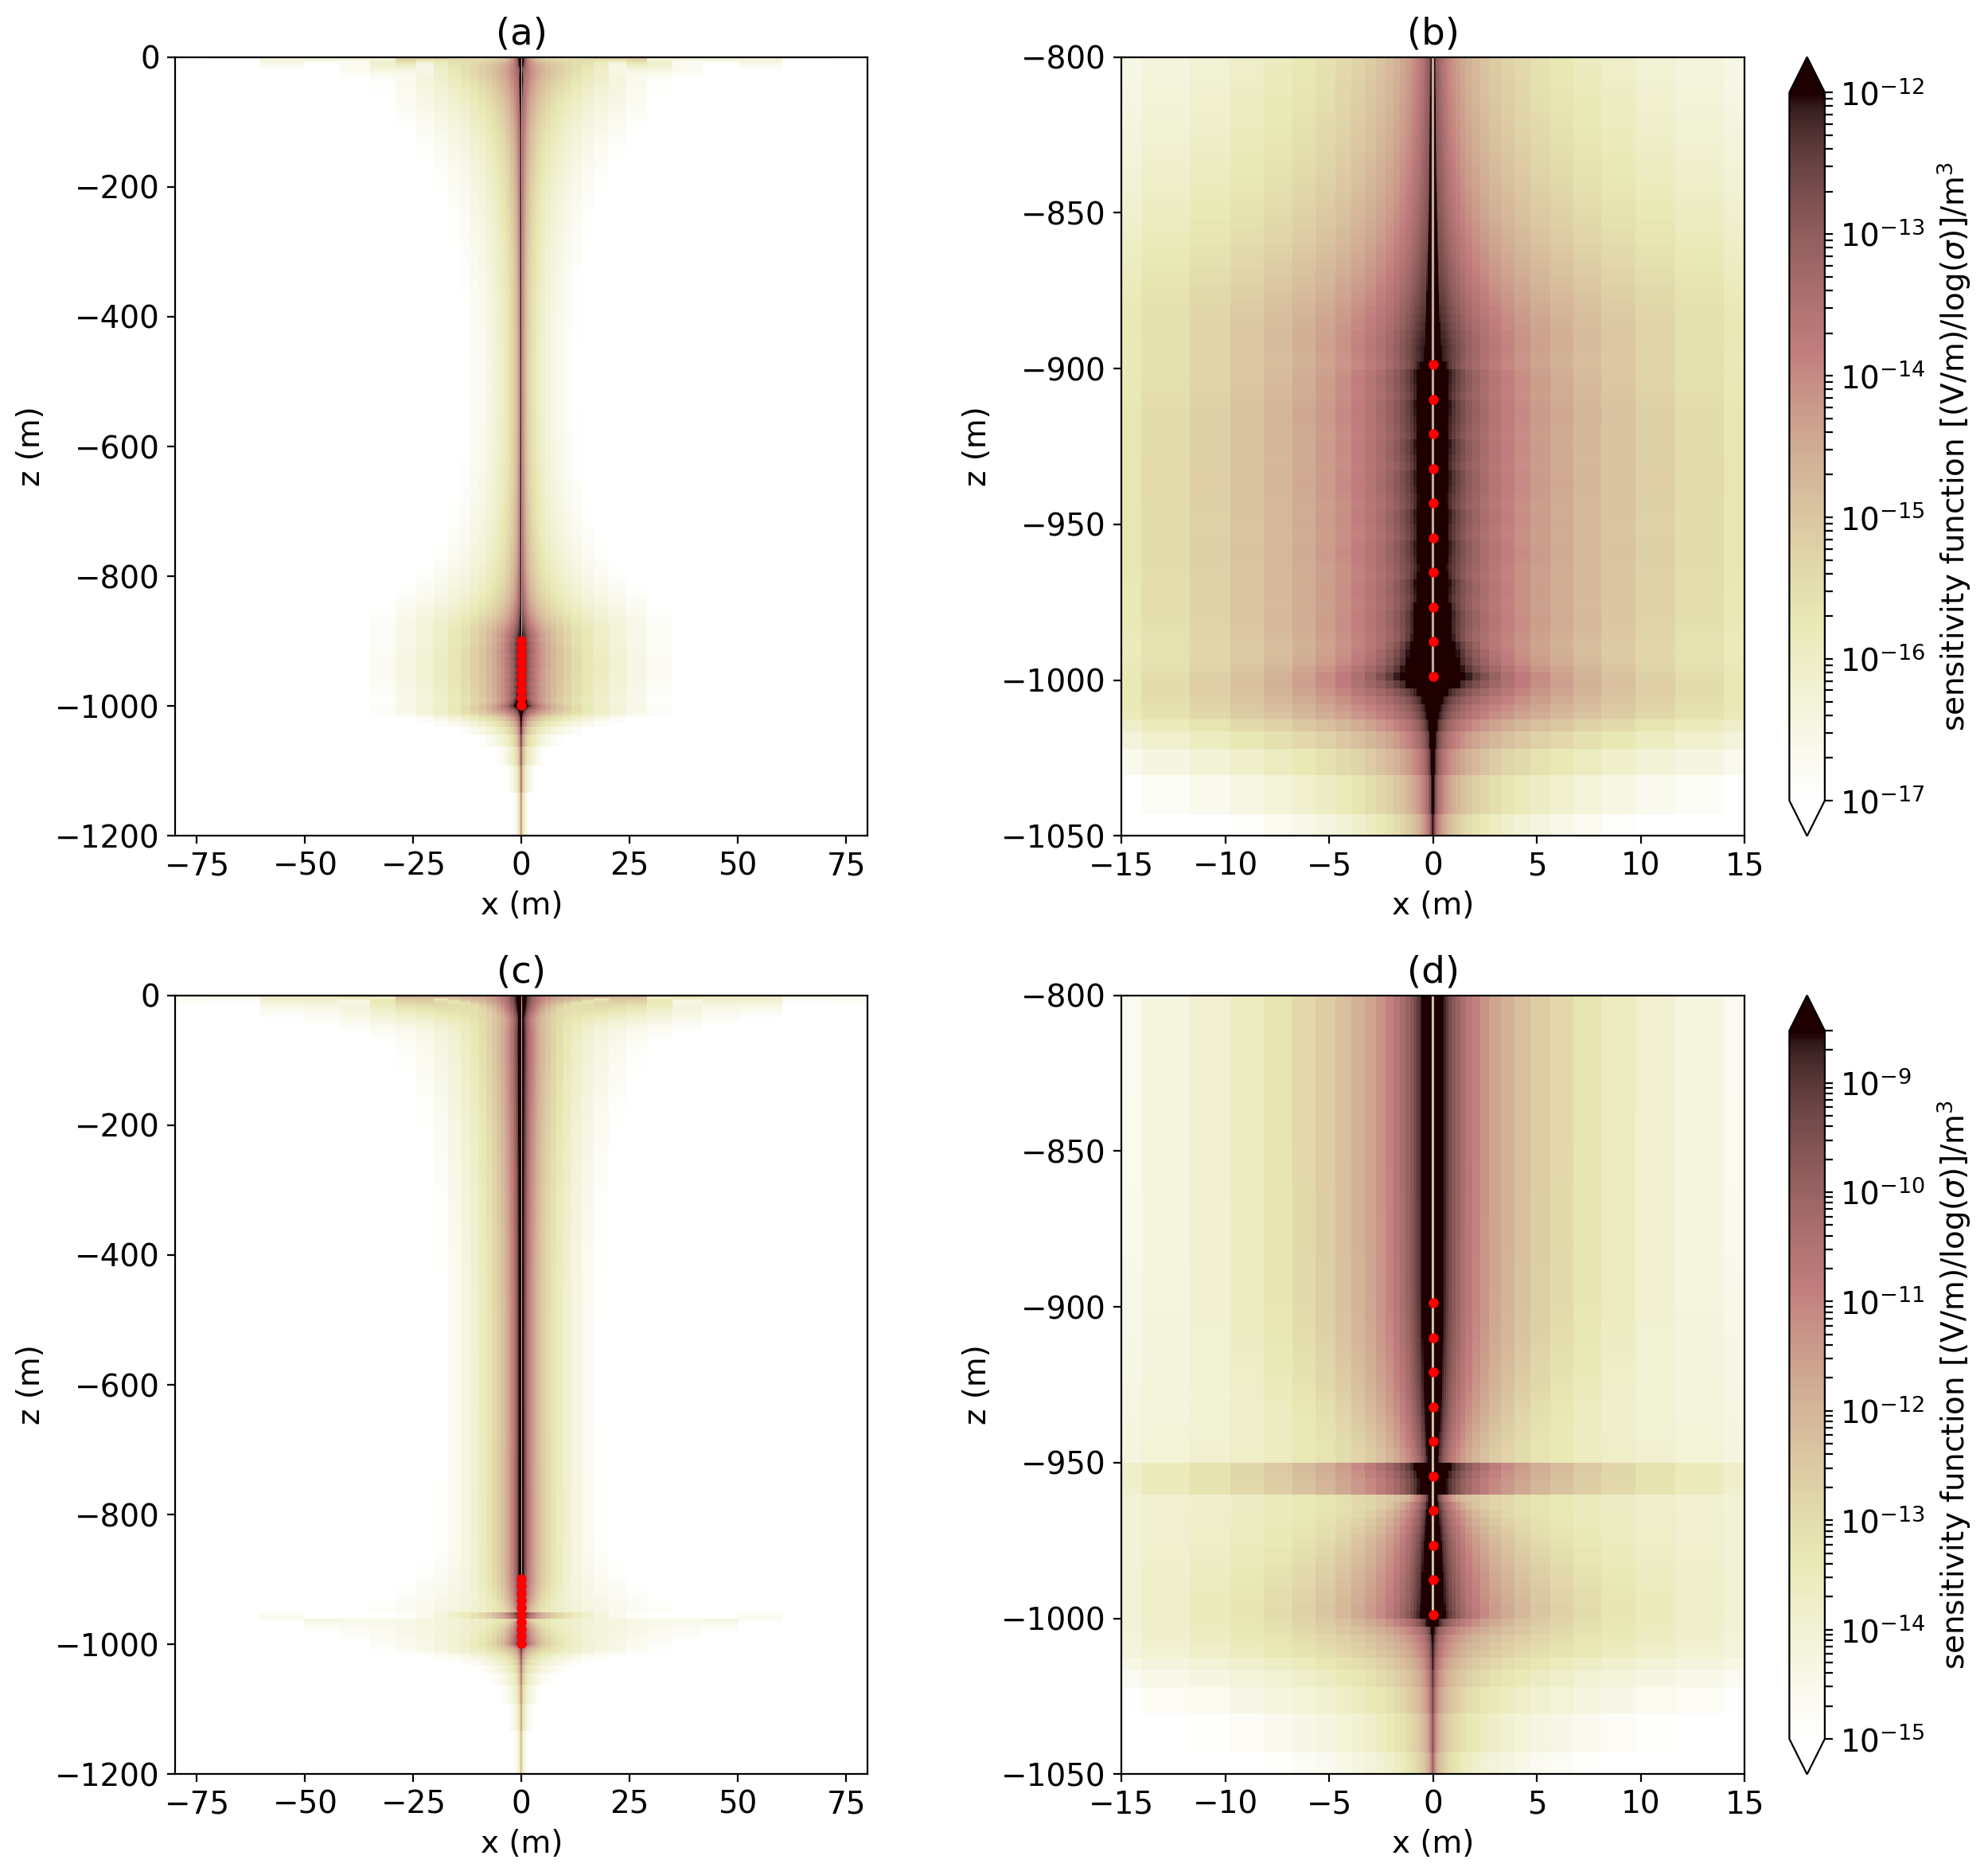
\includegraphics[width=\textwidth]{figures/inversion/casing_sensitivity.png}
    \end{center}
\caption{
    Integrated sensitivity for (a, b) a survey conducted in a 100 $\Omega$m half-space and
    (c, d) the true model with the conductive target, shown in Figure \ref{fig:DC_cyl_setup}.
    The inversion model is log-conductivity.
    The casing is
    shown by the grey line, and the source locations are shown by the red dots. The integrated sensitivity
    is computed by squaring the elements of the sensitivity matrix, summing along the rows of the sensitivity
    matrix and then taking the square-root. This gives a vector whose length is the number of model parameters.
}
\label{fig:casing_sensitivity}
\end{figure}
